\chapter{Tecnologie e Servizi}

\section{Docker}

Docker è diventato negli anni il sistema più popolare per gestire la virtualizzazione basata su container. Può essere visto come un tipo di macchina virtuale leggera, in quanto riesce a garantire le stesse caratteristiche di quelle tradizionali, ma con un overhead minore, sia in termini di efficienza nell'esecuzione, che di spazio occupato. 

\begin{figure}[htbp]
    \centering
    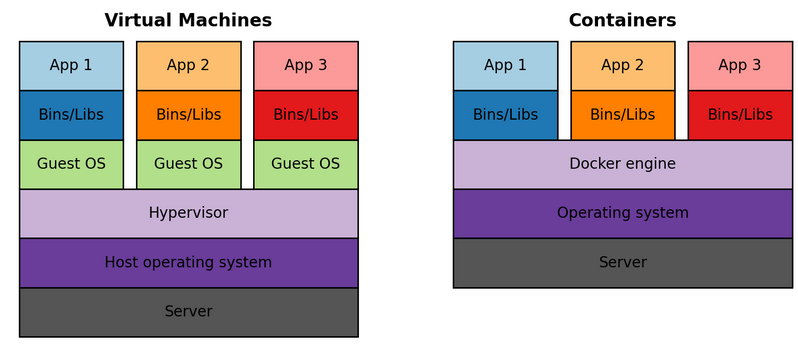
\includegraphics[width=0.9\textwidth]{figures/containers-and-vms.png}
    \caption{Confronto tra macchine virtuali tradizionali e containers.} 
    \label{fig:virt-tech}
\end{figure}

Essi vengono eseguiti direttamente sul sistema operativo dell'host, senza la necessità di chiamate di sistema multiple. Vengono impacchettate solo le librerie necessarie nell'immagine di base fornita al container. In realtà, la sua value proposition è legata alla possibilità di poter lanciare una applicazione ovunque, con la garanzia che questa funzioni sempre. L'analogia con i container nel mondo reale è diretta: quelli utilizzati nel commercio, possono essere adattati indipendemente dall'ambiente di trasporto. Allo stesso modo l'applicazione che viene eseguita, funzionerà indipendemente dall'ambiente di esecuzione, qualsiasi sistema operativo esso sia, con l'unica limitazione sull'instruction set per cui è stata generata la build.  Nella pratica, quindi, esistono due definizioni in base all'utilizzatore di questa tecnologia: se si parla di gestione di una infrastruttura, allora l'attenzione è spostata verso la virtualizzazione, mentre se il focus è relativo alle applicazioni, allora si può vedere Docker come una tecnologia orientata alla portabilità. In generale, le macchine virtuali devono garantire un serie di proprietà per poter essere definite tali, che sono:

\begin{itemize}
	\item \textbf{consolidamento}: inizialmente ciascuna applicazione veniva eseguita su una macchina distinta, rendendo l'utilizzo delle risorse inefficiente. La virtualizzazione ha permesso di superare questa limitazione, con l'esecuzione di software differenti all'interno della stessa macchina.
	\item \textbf{isolamento}: questa proprietà consente ad ogni applicazione di vedere l'ambiente come se fosse una macchina a sé stante, nonostante il consolidamento. I sistemi operativi offrono funzionalità di isolamento base come l'astrazione dello spazio di indirizzamento di un processo, ma questo non è sufficiente per una applicazione self-contained. Diversi applicativi infatti possono interferire tra di loro già solo nell'utilizzo della memoria, nel caso di sovra-allocazioni, portando ad un degrado delle prestazioni o al crash(verifica). Lo stesso ragionamento si può applicare anche per la gestione della cpu, della rete e del filesystem che all'interno di un sistema operativo sono risorse completamente condivise tra processi. 
	\item \textbf{flessibilità}: il controllo dei container è molto semplice in quanto docker prevede dei comandi standard per la loro gestione, come l'avvio, la pausa e lo stop. Gli orchestratori giocano un ruolo fondamentale per riallocare i container in nodi diversi dell'infrastruttura, per esempio in caso di manutenzione o sovraccarico. Questo processo avviene senza particolari overhead, in quanto i container, a differenza delle macchine virtuali tradizionali hanno dei tempi di attivazione molto bassi.
	\item \textbf{portabilità}: come già visto, i container possono essere avviati in qualsiasi piattaforma, indipendemente dal sistema operativo, dall'hardware, dalle librerie necessarie e dalle loro versioni. Questo comporta un grande vantaggio anche nell'uso di linguaggi di programmazione di basso livello quando l'efficienza è fondamentale. Linguaggi come Java, ad esempio, si servono di macchine virtuali per poter garantire la portabilità del codice, ma il tempo di esecuzione aumenta notevolmente. 
\end{itemize}

L'implementazione dei container è stata possibile grazie a due elementi presenti all'interno dei sistemi operativi: namespaces e control groups(cgroups). Si tratta di features che inizialmente non erano state pensate per la virtualizzazione, ma solo nell'ottica di avere dei processi isolati. Non si è quindi arrivati subito alla definizione di container, ma ci sono state delle tappe risolutive di diversi problemi che gli sviluppatori avevano all'inizio degli anni 2000. I namespaces permettevano la gestione della visibilità relativa alle risorse per ogni processo, mentre i cgroups servivano a limitare l'utilizzo di quanto allocato. Nel secondo caso, esistevano già dei meccanismi di questo tipo all'interno del kernel Linux (e.g. cpulimit, nice), ma non erano centralizzati e potevano essere applicati solo a singoli processi. L'evoluzione dei cgroups è fondamentalmente quella di estendere il tutto ad un gruppo di task in maniera modulare, con la possibilità di definire delle gerarchie nella gestione delle risorse. Le tecnologie basate su container come Docker hanno integrato questi meccanismi nel loro layer di virtualizzazione, in modo tale da fornire delle primitive di alto livello per la gestione dei container, che altrimenti con le precedenti astrazioni sarebbero accessibili solo ad utenti esperti, ed in ogni caso inclini ad errori a causa della complessità di utilizzo. 

Docker presenta infine una particolarità a livello di filesystem: rispetto alle macchine virtuali tradizionali o container LXC, che sfruttano un filesystem in senso stretto, questa tecnologia utilizza il concetto di Union Filesystem. 

\begin{figure}[htbp]
    \centering
    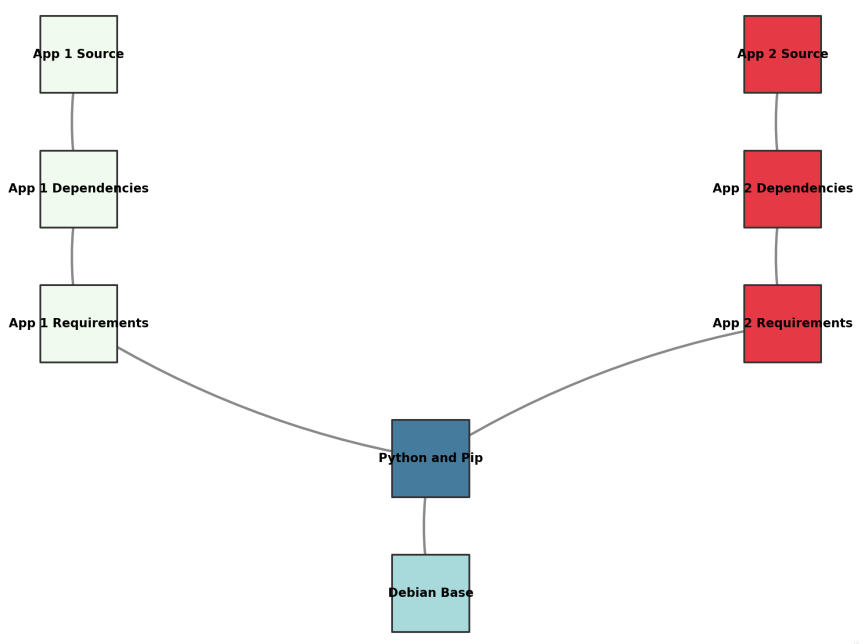
\includegraphics[width=0.69\textwidth]{figures/docker-image-layers.png}
    \caption{Esempio di condivisione di layers in Docker. Le due immagini risultanti hanno la stesso sistema di base, condividendo lo stesso ambiente (Debian) e runtime (Python).}
    \label{fig:image-layers}
\end{figure}

Si tratta di un sistema che combina diversi filesystem restituendo logicamente un'unica struttura. Nell'implementazione di Docker, lo Union Filesystem si presenta come una gerarchia di strati, tutti in sola lettura, a cui ne viene aggiunto uno scrivibile al lancio del container. Questo meccanismo, come si può vedere in Figura \ref{fig:image-layers} permette la condivisione della stessa immagine di base, evitando allo stesso tempo di dover duplicare lo spazio di memoria e che modifiche da parte di una macchina possano influenzare ciò che vedono gli altri container basati sulla stessa istanza, attuando così un primo livello di isolamento (quello più generale con l'host viene sempre implementato attraverso i namespaces). 

La realizzazione pratica di questa funzionalità è possibile grazie al concetto di copy-on-write, già utilizzato nella creazione dei processi. In questo caso il funzionamento è analogo, ma si applica a livello di memoria secondaria. Ogni modifica all'immagine di base, attraverso il layer in scrittura di più alto livello, è ciò che viene salvato. Non si apportano modifiche all'intera memoria: in pratica è un meccanismo basato sulle differenze. Una volta che si esegue il commit di un'immagine, gli strati vengono congelati e ne formano una nuova. Al livello dell'utilizzatore questo sistema si rivela molto utile perché si possono comporre nuove immagini impilando nuovi layer a quelli già esistenti, senza preoccuparsi dei livelli sottostanti, perché grazie alla portabilità il loro funzionamento è garantito. La composizione non è l'unica proprietà interessante che emerge da questa architettura, ma anche modularità, riutilizzo ed efficienza. Quest'ultima è importante sia in termini di spazio, perché come già visto i layer inferiori vengono condivisi, sia in termini di tempo. Quando si costruisce una nuova immagine, infatti, verranno aggiunti o scaricati solo gli strati di più alto livello per la generazione della nuova immagine, invece di dover ri-eseguire l'operazione ogni volta.
  	
\section{MQTT} %mancano definizione esplicita del protocollo, ma emergono nelle responsabilità del broker; subscribe, unsubscribe
Message Queue Telemetry Transport (MQTT) è un protocollo orientato ai messaggi, basato su TCP, il cui obiettivo è quello di fornire un protocollo leggero, per dispositivi con risorse limitate e connessioni instabili. Il formato dei dati infatti è semplice ed è pensato per essere affidabile e fault-tolerant. Proprio per le sue caratteristiche, con il tempo è diventanto uno standard nelle le applicazioni IoT, ad esempio monitoraggio remoto e raccolta di dati in industria, domotica e ambiente. MQTT si basa su un'architettura publish-subscribe. Ciò permette di disaccoppiare l'invio dei messaggi tra produttori e consumatori, attraverso un broker. Si tratta di un metodo di comunicazione indiretto, in quanto per chi pubblica non è necessario conoscere la destinazione, come invece avviene nelle architetture client-server. Il funzionamento è analogo a quello delle newsletter. Quando un utente è interessato ad un certo argomento, lascia il proprio indirizzo email, in modo tale da ricevere aggiornamenti. Analogamente in un sistema publish-subscribe le entità che devono ricevere determinati messaggi da un publisher, si iscrivono ad un canale. 

\begin{figure}[htbp]
    \centering
    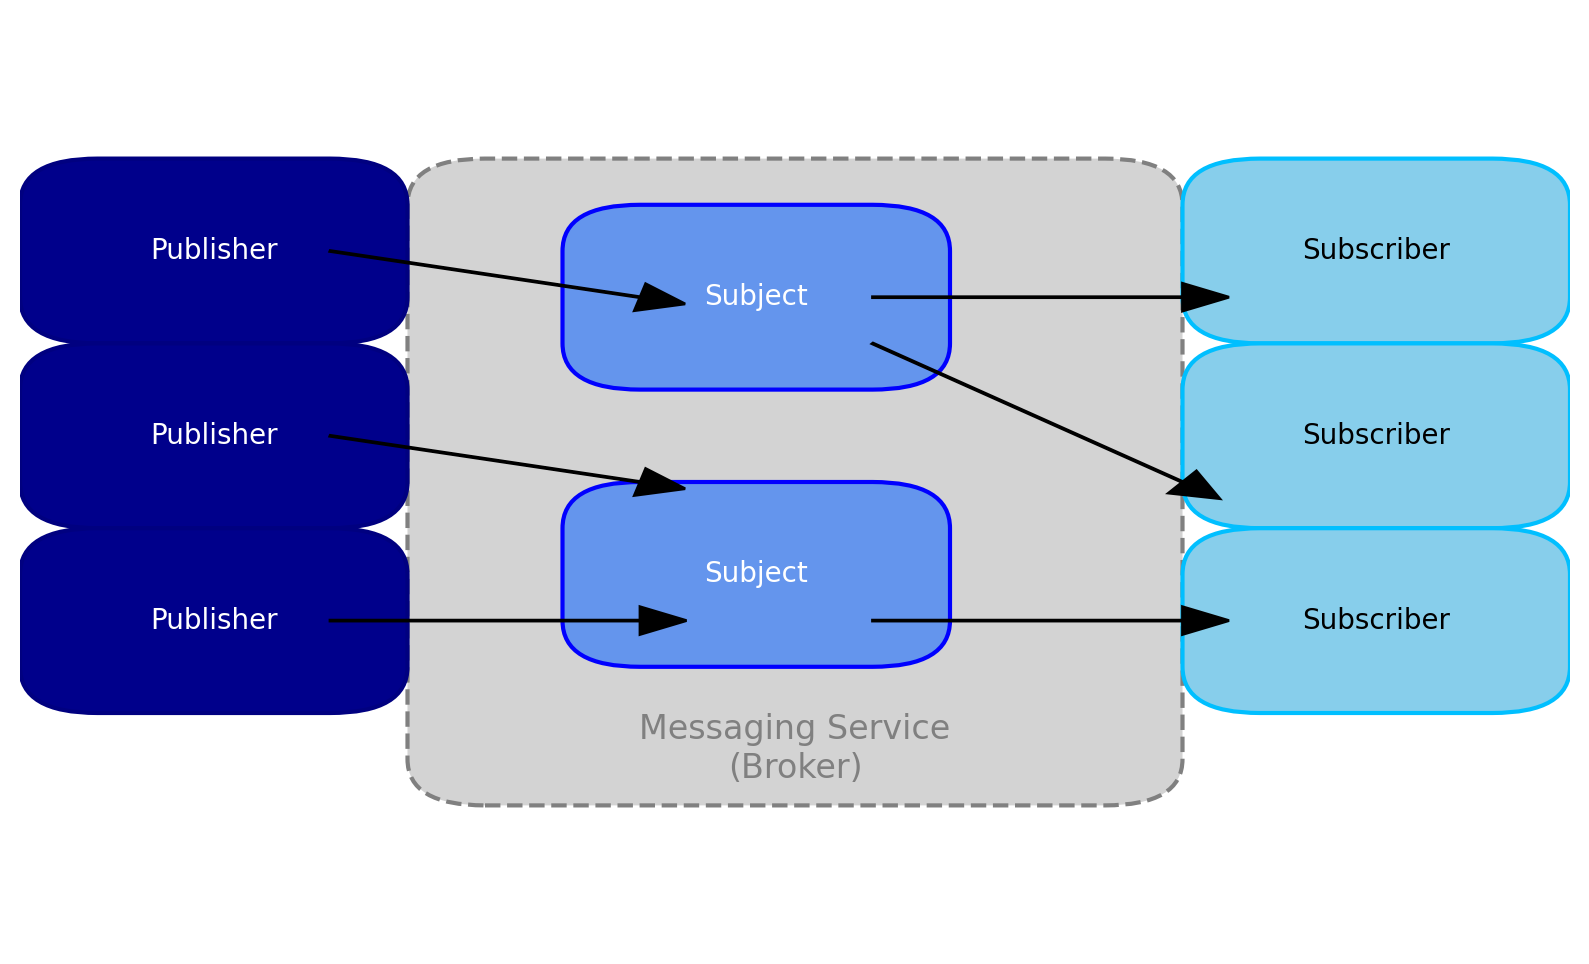
\includegraphics[width=0.63\textwidth]{figures/pub-sub-arch.png}
    \caption{Schema architettura publish-subscribe.}
    \label{fig:pub-sub}
\end{figure}

Oltre al disaccoppiamento, questo tipo di pattern fornisce ulteriori vantaggi\cite{a7IoT4Arch}. E' possibile aggiungere nuovi publisher o subscriber senza dover modificare la logica esistente, il che rende l'architettura facilmente scalabile. Si tratta di uno dei motivi per cui il cloud riesce a gestire facilmente milioni di messaggi in un breve intervallo di tempo ed avere migliaia di publishers. Inoltre ogni parte del sistema non dipende dalle altre, favorendo la comunicazione asincrona, poiché nessun publisher deve aspettare per l'invio di nuovi messaggi prima che i consumatori finiscano. Allo stesso modo i consumatori non devono attendere che altri ricevano i messaggi per poter proseguire con l'elaborazione delle proprie informazioni. Questo tipo di pattern viene implementato in tanti sistemi come quelli delle notifiche push nelle applicazioni mobili, nei servizi gestiti del cloud ed infine nei sistemi IoT, attraverso il protocollo MQTT, focus dei paragrafi successivi. In questo contesto, le unità di interesse vengono descritte come topic. Essi sono univocamente definiti all'interno dei broker attraverso una struttura gerarchica che ricorda i path nelle URI. Ad esempio, un topic può essere dichiarato come: \texttt{factory/floor/sensor1}. Non esiste un meccanismo esplicito di creazione dei topic, ma vengono definiti contestualmente alla pubblicazione di un messaggio.

Il broker ha la responsabilità di connettere, se autorizzati, i diversi client della rete, di tenere traccia dello stato di connessioni precedenti e di filtrare i dati in arrivo dai publisher. Per il discorso di efficienza previsto da questo protocollo, infatti, devono essere distribuiti solo i pacchetti necessari al funzionamento del sistema, e quindi la capacità di filtro è un elemento fondamentale. In particolare, esistono diverse tipologie di controllo dei pacchetti in transito. Quello più importante è il topic filter, dove un messaggio deve contenere necessariamente un topic nell'header, e sarà compito del broker ritrasmetterlo o ignorarlo in base a come è stata implementata la sua logica. In generale i filtri vengono usati per riferirsi ad un insieme di topic, sfruttando due tipologie di wildcards. Si utilizza il segno "+" per indicare un intero livello nella gerarchia del path definito dal topic. Ad esempio \texttt{factory/+/sensor1} serve per tutti i sensor1 nei diversi piani di una fabbrica. Il secondo simbolo, cioè "\#" si riferisce ad una intera sottogerarchia nel path. \texttt{factory/\#} e \texttt{factory/first/\#} filtrano rispettivamente tutti i messaggi provenienti dalla fabbrica e quelli provenienti dal primo piano di un complesso industriale. 

MQTT è un protocollo progettato con l'affidabilità in mente: in base al contesto (hardware, banda, latenza) e al tipo di applicazione, fornisce diversi livelli di Quality of Service(QoS):

\begin{itemize}
	\item \textbf{QoS0}: modalità di funzionamento default in MQTT, se non specificato. I messaggi vengono inviati con una logica fire-and-forget, senza la garanzia che il processo vada a buon fine. Il publisher o il broker inviano i messaggi senza alcun tipo di risposta da parte di un subscriber. Non ci sono ulteriori garanzie oltre a quelle fornite dal protocollo TCP.
	\item \textbf{QoS1}: garantisce che il messaggio venga inviato almeno una volta. Questo meccanismo si basa su messaggi di acknowledgment provenienti dal ricevente, per cui se non arriva nessuna risposta, il messaggio deve essere ritrasmesso.
	\item \textbf{QoS2}: si tratta del livello di qualità più alto. Il messaggio viene inviato una sola volta, grazie ad una serie di messaggi di controllo generati dalle entità in gioco. Può essere visto come un acknowledgement incrociato tra publisher e ricevente. Quello che avviene in più rispetto a QoS1 è l'invio dei pacchetti publish-realease per indicare il rilascio del messaggio dalla memoria del publisher, e publish-complete da parte del ricevente per chiudere la comunicazione. In questo modo alla fine del processo il messaggio è stato inviato e gli attori in gioco sono totalmente sincronizzati dal punto di vista della ricezione.   
\end{itemize}

\begin{figure}[htbp]
    \centering
    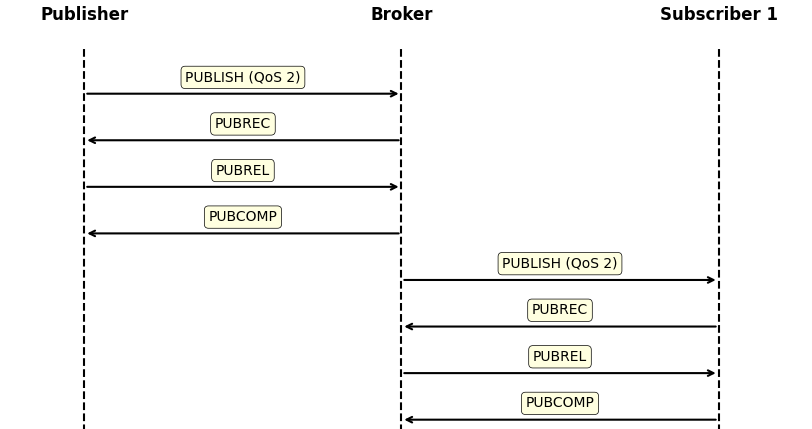
\includegraphics[width=0.9\textwidth]{figures/qos2.png}
    \caption{Flusso pacchetti di controllo per QoS2. I livelli più semplici funzionano in maniera simile, con un numero di pacchetti inferiore. Si può notare come il disacoppiamento fornito dal broker faciliti lo scambio dei messaggi.}
    \label{fig:qos2}
\end{figure}





Il QoS viene negoziato al momento della connessione con il broker, ed in base alle sue capacità può essere dinamicamente modificato in un secondo momento. Nell'affrontare il concetto di qualità di servizio, si è visto quindi il funzionamento della publish da parte di un client, ma esistono altri tipi di operazioni in questo pattern, cioè subscribe, unsubscribe e ping. In particolare quest'ultimo risulta fondamentale per l'implementazione del Last Will and Testament(LWT), un metodo per comunicare la disconnessione di un publisher all'interno della topologia. LWT è un messaggio contente il topic, il QoS e un payload da inoltrare a tutti i subscriber che fino a quel momento ricevevano le notifiche. Questo pacchetto viene fornito nel momento in cui un client si connette per la prima volta al broker, prima che inizi l'invio effettivo dei dati per gli altri client. Se attraverso delle operazioni di ping, impostate con un certo timer, una delle due parti non riceve risposta, allora si assume esserci stata una disconnessione. A quel punto, se è il client ad essere offline, il broker invierà il Will ai subscribers. Un'ultima caratteristica importante per il funzionamento di MQTT, è la persistenza. Il broker mantiene le informazioni di sessione per i client disconnessi, in modo tale da riottenere facilmente le iscrizioni ai topic e i messaggi in coda che non avevano ricevuto (se si tratta di QoS1 e QoS2, pensati come già visto per la trasmissione affidabile). Inoltre, i publisher possono impostare un flag RETAINED nei messaggi, in modo tale che vengano salvati in maniera indefinita nel broker. L'obiettivo di questa funzionalità è garantire l'invio di un determinato messaggio ad un client indipendetemente dal momento della sua iscrizione al topic.  

\section{Protocolli di streaming}
La rete IP è nata per la trasmissione di dati in zone geograficamente distanti tra loro. Le comunicazioni inizialmente erano basate sull'invio di file ed e-mail. La naturale estensione di questo meccanismo è stata quella di poter trasferire informazioni multimediali come animazioni, voce e video in tempo reale, il che ha comportato l'introduzione di nuovi requisiti nello stack IP. Se da un lato il protocollo di livello 3 era sufficiente per le comunicazioni più semplici, esso risultava inaffidabile sia in termini di mantenimento di informazioni, che di ordine di arrivo. L'introduzione del livello TCP ha risolto questa limitazione, ma con l'avvento dello streaming si sono presentati nuovi problemi, legati soprattutto alla latenza e al jitter, rispettivamente il tempo totale per la trasmissione di un pacchetto e la variabilità del delay. 

\begin{figure}[htbp]
    \centering
    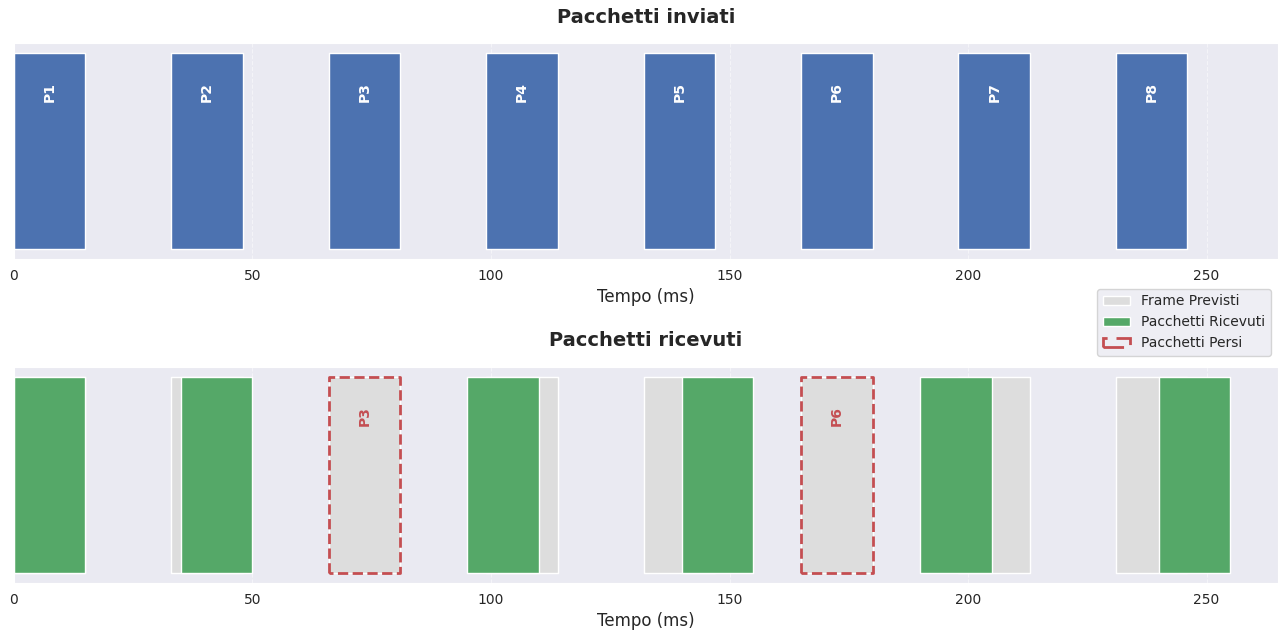
\includegraphics[width=0.9\textwidth]{figures/jitter.png}
    \caption{Effetto del jitter nella riproduzione dello streaming. Senza buffering i pacchetti non vengono riprodotti seguendo la stessa temporizzazione della sorgente.}
    \label{fig:jitter}
\end{figure}

Esistono 2 principali tipologie di software in questo contesto: interattivi (video-conferenze) e passivi (live-streaming). Nel primo caso i requisiti sul ritardo
e sul jitter sono molto stringenti, per cui non si possono introdurre meccanismi pesanti di bufferizzazione, poiché compromettono irrimediabilmente la user experience. Possono invece essere implementati nel secondo, in modo tale da mitigare gli effetti della trasmissione. Bisogna ridurre al minimo i tempi di attesa: ad esempio il reinvio dei pacchetti, come succede in TCP, non può essere implementato. UDP invece si presta a questo meccanismo ed infatti fornisce la base per un protocollo di streaming in tempo reale. Non instaura nessun tipo di connessione e non deve monitorare le condizioni della rete per adattare la sua velocità nella comunicazione. Real-time Transport Protocol(RTP) è un protocollo di livello trasporto \cite{a8rfc3550}%rfc3550 lo pone esattamente sul trasport layer("both protocols contribute parts of the transport protocol functionality") 
è stato progettato per lavorare sopra UDP, e con le sue caratteristiche è in grado di soddisfare i requisiti per la trasmissione di dati multimediali su internet. RTP infatti permette la negoziazione di una codifica comune ai lati della comunicazione. Grazie a questo protocollo, i livelli applicativi sono liberi di implementare il buffering in base alle proprie necessità, poiché integra nei pacchetti il timestamp del contenuto multimediale. RTP non è sensibile al livello di congestione della rete, quindi il rate di trasmissione non viene modificato, come invece succede in TCP. %Si può tuttavia operare sul jitter, tramite riordinamento e buffering: se la variabilità nell'arrivo dei pacchetti porta ad una trasmissione fuori ordine, è possibile grazie alla bufferizzazione, a livello applicativo, risolvere questo problema. Inoltre, sempre grazie a questo meccanismo, si possono riprodurre i dati secondo il loro naturale timestamp, proprio perché questa informazione viene codificata nel protocollo di fatto utilizzato per le trasmissioni streaming in internet: Real-time Transport Protocol (RTP). 2. c'è da parlare anche del fatto che lo scarto di alcuni pacchetti non porta al degrado totale della user experience, ma in base allo use case e allo stato della rete si possono in qualche modo saltare dei pacchetti (un po' emerge quando si parla di sequence number).

RTP lavora in coppia con Real-time Control Protocol (RTCP), la sua controparte per la verifica dello stato della rete. A differenza di TCP, questo protocollo ha una funzione di solo monitoraggio, non serve per reagire alle congestioni, quindi ai ritardi, alle perdite o al jitter. Si tratta di un protocollo leggero, che periodicamente invia messaggi di controllo verificando lo stato della rete, in modo tale che i livelli applicativi, in base alla qualità che vogliono fornire, reagiscano di conseguenza. Si è delegato quindi al software questo onere, senza fornire una maniera standard per il controllo del traffico. Questo è un grosso vantaggio in termini di flessibilità: sfruttando TCP al contrario, la velocità di trasmissione dipenderebbe dalle sue regole nella gestione del flusso di informazioni. Esiste infine un protocollo di più alto livello per la gestione delle sessioni nella trasmissione dati: Real-time Streaming Protocol (RTSP). Esso non invia i pacchetti effettivi per lo streaming, perché svolto interamente da RTP, ma una volta che la sessione è attiva, serve per inviare i comandi relativi allo stato di quest'ultima. Per cui il client che richiede dati multimediali manderà al server dei messaggi per avviare, sospendere o fermare il flusso di informazioni.

%rtp: protocollo di trasporto dati
%rtcp: protocollo di controllo di stato dello streaming
%rtsp: protocollo di controllo della SESSIONE di streaming 

\begin{figure}[htbp]
    \centering
    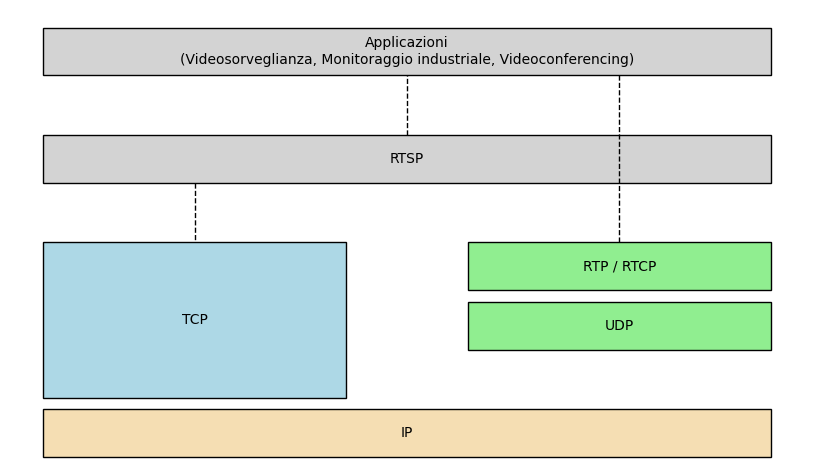
\includegraphics[width=0.9\textwidth]{figures/streaming_stack.png}
    \caption{Stack di protocolli per lo streaming real-time.}
    \label{straming-stack}
\end{figure}

Il formato dell'header RTP è costituito da tre elementi principali. I primi 12 bytes sono sempre presenti e formano il core del pacchetto. Successivamente possono esserci delle estensioni (anche se usate molto raramente) ed infine c'è il campo payload, il cui formato è deciso dall'applicazione. Nel dettaglio i campi di RTP sono:

\begin{itemize}
	\item \textbf{version}: bit per l'identificazione della versione di RTP usata nella trasmissione. 
	\item \textbf{padding}: se questo campo è configurato, sarà presente del padding nel pacchetto, ad esempio per allineamento oppure se si sta utilizzando qualche algoritmo di cifratura. 
	\item \textbf{extension}: quando il bit è attivo, il campo extention header sarà presente nel pacchetto. 
	\item \textbf{CSRC Count}: conta il numero di sorgenti multiple, quando sono presenti, come spiegato nel campo CSRC. 
	\item \textbf{marker}: identifica punti specifici nel flusso multimediale, come i confini tra diversi frame in un video.
	\item \textbf{payload type}: campo per la decodifica del contenuto multimediale nel payload.
	\item \textbf{sequence number}: numero identificativo del pacchetto. E' utile per stabilire se ci sia stata una perdita e permettere alle applicazioni di reagire. Queste possono decidere di non procedere in nessun modo oppure di attuare delle strategie. Ad esempio si potrebbe utilizzare delle codifiche che richiedono meno banda o riprodurre il frame precedente/successivo più volte.
	\item \textbf{timestamp}: indica il momento di generazione del pacchetto attraverso il clock di sistema. Serve per sincronizzare i flussi audio e video. Viene inoltre utilizzzato per determinare il jitter.
	\item \textbf{Synchronization Source Identifier(SSRC)}: identifica la sorgente nella comunicazione RTP. E' un valore scelto in randomicamente a livello locale dalle fonti, quindi esiste la possibilità di collisioni. In tal caso RTCP non permette che questo evento si verifichi, facendo uscire e rientrare dalla sessione una delle due sorgenti.
	\item \textbf{Contributing Source Identifiers(CSRC)}: è una lista delle sorgenti che contribuiscono al payload del pacchetto, anche se in generale il source è solitamente uno solo. E' utile nel caso delle videoconferenze quando più fonti generano un stream di dati, ma si vuole compattare i flussi in un unico pacchetto per necessità di banda. 
\end{itemize}

In RTP non è presente un concetto esplicito di sessione, ma esso viene definito contestualmente alla generazione dello streaming, idenficando il destinatario tramite indirizzo IP e una coppia di porte RTP ed RTCP. %potrebbe aver senso parlare delle sessioni multimediali dove ad esempio viene gestito audio e video contemporaneamente. In quel caso si generano due flussi RTP e l'applicazione poi decide se usare entrambi i flussi o solo uno. In questo contesto si potrebbe introdurre il mixing. 

RTSP è nato come standard per la definizione delle sessioni multimediali ed il loro controllo. %nel caso di mqtt manca una trattazione approfondita della subscribe, qui manca per RTCP. 
In RFC2326 è definito come "remote control" nella gestione dello streaming, perché si presenta con una serie di comandi, che ricordano molto quelli di HTTP. Tuttavia differisce da questo protocollo in un punto fondamentale: RTSP è simmetrico, in quanto sia il client che il server multimediale possono inviare richieste. Inoltre i messaggi non sono di tipo fire and forget, infatti i comandi inviati possono riferirsi a richieste precedenti, rendendo di fatto RTSP un protocollo stateful\cite{a9rfc2326}. %specificare che gli stream vengono fatti su http, ma nel monitoraggio e nelle applicazioni industriali, dove i requisiti di latenza sono più bassi RTSP viene ancora utilizzato. Quale protocollo è più veloce tra RTP e WebRTC? 2. la simmetria di RTSP è specificata nel suo RFC. 3.segue qua sotto una cit da mio fratello in cristo durresi.
Non è un meccanismo orientato alle connessioni, per cui anche appoggiandosi a TCP potrebbe più volte aprire diverse comunicazioni attraverso il protocollo di livello trasporto nella stessa sessione RTSP. In generale il suo funzionamento non dipende dal protocollo di livello 4 sottostante, per cui si può appoggiare sia a TCP che ad UDP nella generazione dei propri messaggi, ma tipicamente viene utilizzato TCP. Nonostante i requisiti di bassa latenza per l'intero sistema di streaming, nel caso di RTSP è importante che i comandi arrivino a destinazione, per cui si utilizza un canale di comunicazione affidabile, separato dal flusso vero e proprio. Questo non comporta degrado delle prestazioni perché i pacchetti sono su un canale separato e la quantità è talmente limitata che non impatta sulla banda disponibile. Infine, per quanto riguarda le sue caratteristiche, bisogna menzionare come vengono identificati gli stream. Si sfrutta un RTSP URL (e.g. \texttt{rtsp://hostname/video/front}), in maniera molto simile a come vengono definite le risorse in HTTP. Questo mapping è molto utile perché può applicare i comandi a più stream contemporaneamente, seguendo la struttura gerarchica dei path nell'URL. Ad esempio se ci sono più flussi video, come \texttt{rtsp://hostname/video/front} e \texttt{rtsp://hostname/video/top}, inviando un comando a \sloppy\texttt{rtsp://hostname/factory/video}\fussy, questo si applicherà ad entrambe le risorse. %<---appendice dell'rfc
I metodi disponibili in RTSP sono:
\begin{itemize}
	\item \textbf{OPTIONS}: insieme dei comandi che entrambe le parti possono accettare, serve quindi per verificare la compatibilità delle operazioni disponibili tra gli estremi di comunicazione.
	\item \textbf{DESCRIBE}: questo comando fornisce la descrizione del contenuto multimediale come il formato e la codifica. 
	\item \textbf{SETUP}: inizializza la sessione di streaming RTSP, tramite dei parametri (e.g. porta, protocollo di trasporto) dopo che entrambe le parti hanno allocato le risorse necessarie.
	\item \textbf{PLAY}: il client invia questo comando quando richiede l'effettiva trasmissione del flusso.
	\item \textbf{PAUSE}: lo streaming viene interrotto dal client senza che il server liberi le risorse e i parametri di sessione.
	\item \textbf{TEARDOWN}: il client richiede lo stop dello streaming, seguito dalla liberazione delle risorse nel server.
	\item \textbf{GET\textunderscore PARAMETER, SET\textunderscore PARAMETER}: questa serie di comandi fornisce o imposta i parametri di sessione nello streaming (ad esempio i pacchetti ricevuti, il jitter etc). 
\end{itemize}

RTSP definisce una macchina a stati, che permette la coordinazione del flusso di streaming multimediale, in modo tale da consentire ai partecipanti della sessione di sapere quali comandi possono inviare o ricevere in ogni sua fase. Sia il client che il server memorizzano lo stato della sessione per avere una interazione coerente tra di loro. 

%cerca l'esempio di sessione per la generazione di un flusso infinito. nel caso mettilo qui ed aggiungi un grafico, oppure fallo in appendice. 

%l'introduzione al cloud fornita nel background non è formale ed è stata subito incentrata verso le nuove industrie. quindi puoi dare una definizione più rigorosa di cloud e di aws.
\section{Amazon Web Services}
%introduzione
Amazon Web Services (AWS) è una piattaforma pubblica basata su cloud che offre servizi gestiti per la generazione di soluzioni a diversi livelli di astrazione. Per quanto riguarda lo storage ad esempio, si potrebbe richiedere al provider una macchina virtuale e collegare ad essa un volume, implementando così una soluzione di basso livello. Altrimenti è possibile sfruttare servizi come S3 e salvare le proprie informazioni attraverso una API, ottenendo un risultato simile, ma ad alto livello. La scelta dipende sempre dalle necessità dell'utente, tuttavia l'opzione più facile è sicuramente la seconda, perché con una semplice chiamata si possono salvare le proprie informazioni come se si utilizzasse un filesystem remoto, senza preoccuparsi della gestione interna, della durabilità, delle dimensioni dei file ed in generale della grandezza dello storage, che può scalare teoricamente in maniera indefinita. %livello piattaforma, livello servizi --> descrivi i modelli del cloud (saas,paas,iaas,haas).

Le API sono accessibili attraverso protocolli web, coerente con le caratteristiche fornite da NIST per quando riguarda il cloud computing. Tra queste infatti è presente il concetto di "broad network access", cioè le funzionalità del cloud computing vengono erogate attraverso la rete. Altre proprietà comprendono la possibilità di ottenere i servizi su richiesta da parte dell'utente senza ausili esterni (on-demand self-service), condivisione di un'unica piattaforma da parte degli utenti (resource pooling), risposta rapida alla richiesta di risorse imposte dalla variabilità nel workload (rapid elasticity).  
%geolocalizazione e modello di pagamento.
%benefici
L'adozione del cloud computing viene spesso sponsorizzata per il modello dei costi lato utente, basata sul pay-per-use. Questo significa ridurre le spese nel caso di startup che non possiedono una infrastruttura IT, oppure per aziende che vogliono ricostruire o estendere la propria. Inizialmene può essere un vantaggio, ma bisogna sempre monitorare l'utilizzo e l'archiettura delle proprie soluzioni in modo che i costi operativi non esplodano. In generale quindi il modello introdotto da Amazon può essere considerato un beneficio, tuttavia si tratta del punto di partenza per esplorare ulteriori vantaggi che il provider introduce. 

%1. innovation and integration
AWS è una piattaforma innovativa, che annuncia costantenemente nuovi prodotti. L'implentazione di queste tecnologie viene poi integrata nell'ecosistema esistente, contribuendo al continuo allargamento della piattaforma. %2. common problem resolution
I servizi gestiti forniti dal provider sono pensati per risolvere problemi comuni, in modo tale che il cliente si focalizzi solo sulle soluzioni. Per cui non sarà necessario implementare meccanismi di load balancing o per le notifiche in quanto AWS fornisce queste funzionalità a priori. %3 automation
Il paradigma Infrastructure as Code (IaC) rende la gestione delle risorse automatica: si tratta di un effetto collaterale dell'utilizzo delle API. L'utente deve solo dichiarare le risorse necessarie, non gestire manualmente la loro allocazione. Una volta definite le parti del sistema, sarà compito di AWS invocare i comandi che servono per la loro creazione. %4 scaling
La capacità del cloud si può adattare in proporzione al carico di lavoro, definendo un numero di macchine virtuali in base alla periodicità (giorni, settimane, mesi) e a quando vengono raggiunti i picchi. Basta incrementare il numero di macchine virtuali e quando non saranno più necessarie eliminarle. Questo meccanismo avviene molto velocemente, quindi non si tratta solo di un vantaggio di scalabilità, ma anche di velocità di allocazione e deallocazione delle risorse. %5 relability
AWS offre dei servizi che sono affidabili by default: ad esempio S3 è progettato per avere una durabilità dei dati al 99,9\%. Inoltre vengono forniti strumenti per rendere la propria infrastruttura affidabile, non limitandosi quindi solo ai servizi, ma anche a livello di sistema. La possibilità di poter deployare la propria infrastruttura in più regioni rientra in questa categoria. Oltre ad essere un vantaggio in termini di accessibilità, latenza e protezione dei dati, quando una delle repliche possiede un guasto, si può continuare a garantire il servizio utilizzando il deploy di un'altra regione. Inoltre, sempre nell'ottica dell'affidabilità, vengono forniti dei servizi per il monitoraggio e l'alterting dell'infrastruttura, come nel caso di Amazon CloudWatch e AWS X-Ray. Si possono così controllare le metriche principali come latenza, utilizzo delle risorse e throughput. Nel momento in cui si verificano anomalie si possono poi impostare degli avvisi per reagire tempestivamente agli eventi inattesi. 

%introduzione ai servizi e deep-down a quelli che ho utilizzato
Come si può notare in Figura \ref{fig:services_taxonomy}, i servizi offerti da AWS si dividono in due categorie: hardware e software, basati sull' infrastruttura sottostante\cite{a10AWSinAction}. Poiché in questo lavoro si è sfruttato unicamente il modello PaaS, % o SaaS? Descrivi i modelli in appendice 
il focus della classificazione nell'analisi sarà solo sulla parte software.
%vedi se riesci a produrre un'immagine coerente
\begin{figure}[htbp]
    \centering
    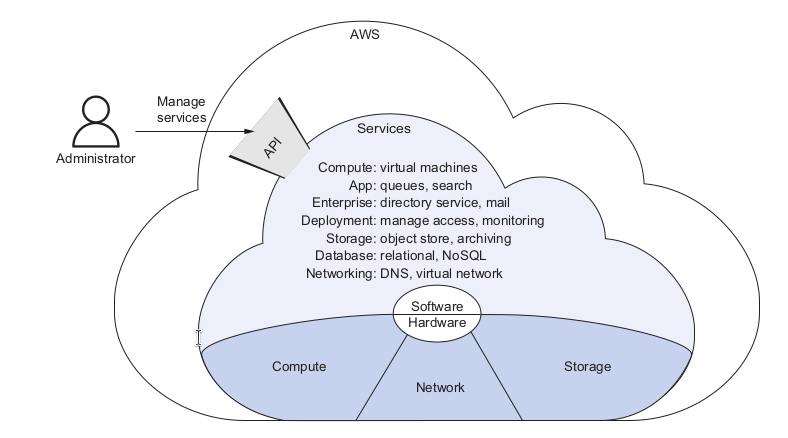
\includegraphics[width=0.59\textwidth]{figures/aws_services_taxonomy.png}
    \caption{Classificazione ad alto livello dei servizi AWS. Accessibili attraverso API, si dividono nelle due macro-aree hardware e software.}
    \label{fig:services_taxonomy}
\end{figure}

Per quanto riguarda la categoria compute, l'obiettivo è quello di fornire rispettivamente servizi per l'esecuzione di applicazioni su macchine virtuali e per la gestione delle risorse di calcolo, come nel caso di Elastic Compute Cloud (EC2). Per app si intendono quei servizi a diretto supporto delle applicazioni, necessari per la risoluzione di problemi comuni, come l'implementazione delle code di messaggi o delle notifiche. I servizi enterprise sono pensati per la gestione delle risorse aziendali, ad esempio Organizations è un tool per il controllo di più account AWS, in modo tale da poter effettuare raggruppamenti in base alle unità nell'organizzazione ed aggregare policy e operazioni per ciascun gruppo. La categoria deployment, come si può facilmente intuire, fornisce strumenti per la distribuzione del software. Storage è l'insieme dei servizi per la memorizzazione dei dati in modo sicuro, scalabile e di lunga durata. Tra questi rientrano sicuramente gli object store come S3 e i servizi di archiviazione a lungo termine e backup come Glacier. Le ultime due categorie riguardano i database (RDS per i relazionali, DynamoDB per quelli non relazionali) ed il networking come Virtual Private Cloud (VPC) per la creazione di reti isolate nel cloud. %mancano networking e database.
In Tabella \ref{tab:aws_services}, infine, viene mostrata la tassonomia, secondo le classi appena definite, dei servizi usati nell'implementazione del sistema di rilevazione dei DPI, con una breve descrizione del loro funzionamento, approfondito nel capitolo successivo. 

\begin{longtable}{@{}p{3cm}p{2.5cm}p{7cm}@{}}
\toprule
\textbf{Servizio} & \textbf{Categoria} & \textbf{Descrizione} \\ \midrule
\endfirsthead

\endhead
%\bottomrule
%\endfoot

%\toprule
CloudFormation & Deployment & Tramite il paradigma Infrastructure as Code, permette la dichiarazione di uno stack con le risorse necessarie ed indica le policy di accesso tra i vari servizi. \\ \midrule
Lambda & Compute & Funzione utilizzata in architetture event-driven, programmata senza dover gestire l'infrastruttura sottostante (macchine virtuali, sistemi operativi). \\ \midrule
IAM Policy & Enterprise & Consente di definire le regole di accesso e autorizzazione tra servizi AWS, rendendo possibili interazioni sicure e controllate. \\ \midrule
Kinesis-Video Streams & App & Gestisce in maniera scalabile l'ingestion di flussi video dall'esterno del cloud e li inoltra a servizi downstream, come S3, EC2 o applicazioni di machine learning (e.g. Rekognition). \\ \midrule
AWS IoT Core e Greengrass & App & Controllano in maniera coordinata lo stato dei dispositivi IoT e inoltrano i relativi messaggi di telemetria provenienti dall'edge. \\ \bottomrule
\caption{Classificazione dei servizi AWS di interesse.} \label{tab:aws_services}
\end{longtable}

%aggiungi tabella con i servizi che hai usato
%introduci parte successiva

%\subsection{Infrastructure as Code}
%\subsection{Serverless}
%\subsection{Iam Policy}
%\subsection{Kinesis Video Streams}
%\subsection{AWS Iot Core e Greengrass}
\section{Apache Flink}
%\section{GStreamer}



